%\documentclass{jpsj3}
\documentclass[fp,twocolumn]{jpsj3}
%\documentclass[letter,twocolumn]{jpsj3}
%\documentclass[letterpaper,twocolumn]{jpsj3}
\usepackage{txfonts}
\usepackage{algorithm}
\usepackage{algorithmic}
\usepackage{amsmath}
\usepackage{multirow}

\makeatletter
\@dblfptop 0pt
\makeatother

\renewcommand{\topfraction}{.85}
\renewcommand{\bottomfraction}{.60}
\renewcommand{\textfraction}{.15}
\renewcommand{\floatpagefraction}{.6}

\title{Derivaton of the QUBO formulation for sparse estimation}

\author{Tomohiro Yokota$^1$%\thanks{jpsj{\_}edit@jps.or.jp}
  , Makiko Konoshima$^2$, Hirotaka Tamura$^2$, Jun Ohkubo$^3$}
\inst{$^1$Graduate School of Science and Enginnering, Saitama University,
  255 Shimo-Okubo, Sakura-ku, Saitama-shi, 338-8570, Japan\\
  $^2$Fujitsu Laboratories Ltd.,
  4-1-1 Kawasaki, Kanagawa 211-8558, Japan
  $^3$JST, PREST, 4-1-8 Honcho, Kawaguchi, Saitama 332-0012, Japan} %\\

\abst{%l1-normのQUBO形式での定式化を提案する. これにより, スパース推定に対するQUBO形式を導出することができるようになる. Sato et al.(2019)が提案したReLUタイプ関数の定式化の方法を応用することで, l1-normのQUBO形式での導出を行なった. 加えて, 数値実験を通して, 定式を見直すことにより変数を減らすことができた.
  We propose the $\ell_{1}$-norm in QUBO formulation, which makes it possible to derive the QUBO formulation for sparse estimation. I derived the $\ell_{1}$-norm in the QUBO formulation by applying the method of formulation of ReLU type function proposed by Sato et al. (2019). In addition, through numerical experiments, I was able to reduce the variables by reviewing the fomulation.
}

%%% Keywords are not needed any longer. %%%
%%% \kword{keyword1, keyword2, keyword3, \1dots} 
%%%

\begin{document}
\maketitle

\section{Introduction}
%近年では, D-Wave Systems Inc.のD-Waveや富士通のデジタルアニーラのようなイジング型マシンの開発が進められている.
In recent years, Ising machines such as D-Wave Inc.'s D-Wave and Fujitsu's Digital Annear have been developed.
%利用できる量子ビット数が年々増加しており, これにより大きな組み合わせ最適化問題に対してイジング型マシンでの計算ができるようになった.
The number of available qubits has been increasing year by year, which has enabled Ising machine calculations for large combinatorial optimization problems.
%しかし, イジング型マシンで最適化問題を計算するためには, コスト関数をQUBO形式に変換しハードウェアとして実装する必要があるが, QUBO形式への系統的な導出方法はまだ見つかっていない.
However, to calculate the optimization problem with Ising machine, it is necessary to convert the cost function into QUBO form and impliment as hardware, but a systematic derivation method to QUBO form has not been found yet.

%先行研究ではq-loss関数とReLUタイプ関数のQUBO形式での導出がされている.
In previous research, $q$-loss function and ReLU type function have been derived in the QUBO form.
%q-loss関数の導出法についてはLegendre変換を適用することでQUBO形式を導出することができた.
As for the derivation method of $q$-loss function, QUBO form could be derived by applying Legendre transformation.
%しかし, ReLUタイプ関数に対しては, Legendre変換だけを適用しただけではコスト関数のmin関数にマイナス符号が付いてしまい複数のコスト関数を組み合わせて最適化問題を解くことができない.
However, for the ReLU type function, the $\min$ function of the cost function has a minus sign only by applying the Legendre transform, and it is impossible to solve the optimization problem by combining multiple cost functions.
%そこで, Wolfeの双対定理を追加で適用することでこの問題を解決した.
Therefore, this problem was solved by additionally applying Wolfe duality theorem.

%本稿で紹介するl1-normはスパース推定を行う際に利用されている.
The $\ell_{1}$-norm introduced in this paper is used in sparse estimation.
%スパース推定はデータ解析や画像処理の分野で利用されている.
Sparse estimation is used in the field of data analysis and image processing.
%データ解析で利用されるもので代表的なものにLassoがあり, 最小二乗法のコスト関数にl1-normを加えることでスパースな推定を行うことを可能にしている.
Lasso is a typical example used in data analysis, and it is possible to perform sparse estimation by adding $\ell_{1}$-norm to the least-squares cost function.
%スパース推定の考え方は, ブラックホールの解析でも利用されている.
The idea of sparse estimation is used in black hole analysis.
%ブラックホールとても小さく, 今までの手法では解像度が低いため観測することが不可能であった.
The black hole is so small that it is impossible to observe it by the previous method because the resolution is low.
%そこで, 世界中の電波望遠鏡から同時に測定を行い, その観測データに対してスパース推定を行うことで本質的な情報のみを取り出しブラックホールの画像化を行なった.
Therefore, we performed simultaneous measurements from radio telescopes all over the world, performed sparse estimation on the observation data, extracted only essential information, and performed imaging of black holes.
%このように, スパース推定をイジング型マシンで行う上でこの研究は重要である.
Thus, this research is important in performing sparse estimation on Ising machines.

%本稿ではl1-normのQUBO形式での定式化を行う.
In this paper, we derivate $\ell_{1}$-norm in QUBO formlation.
%そのために, Legendre変換およびWolfeの双対定理を用いる.
To do this, we use the Legendre transform and Wolfe duality theorem.
%さらに, 定式化を見直すことで, 単純に適用した場合よりも変数を減らせることが確認できた.
Furthermore, it was confirmed that the variables can be reduced by reviewing the formulation, compared to the case of simple application.
%これはイジング型マシンの量子ビット数に制限がある現在において, ハードウェアへの実装を考える上で重要なことである.
This is important when considering hardware implementation in the current situation where the number of qubits of Ising machine is limited.

%本稿の構成は次のようになる.
The composition of  this paper is as follows.
%第二章では, QUBO形式, 先行研究, 導出に利用する定理についての説明を行う.
Chapter 2 explains the QUBO form, previous researchs, and theorems used for derivation.
%第三章では, l1-normのQUBO形式での導出およびその検証を行う.
Chapter 3 carried out the derivation of $\ell_{1}$-norm in the QUBO form and its varification.
%第四章では, 定式化を見直すことで目的関数から変数を削除し, 結果に影響がないかを検証する.
Chapter 4 removes variables from the objective function, and varifies whether the result is not affected.
%第五章では第四章での結果およびこれからの展望について語る.
Chapter 5 discusses the results of Chaption 4 and the prospects for the future.

\section{Background}
In this section, we describes the knowledge.

\subsection{QUBO and Ising model} %QUBOとIsingモデルについての説明
Since the QUBO formulation and the Ising model are equivalent, we can be converted to other form if we can be represented one side. The Ising model is represented as follows:
\begin{eqnarray}
  H=-\sum_{i,j}{J_{i,j}\sigma_{i}\sigma_{j}}-\sum_{i}{h_{i}\sigma_{i}}
\end{eqnarray}
where $\sigma_{i}\in \{-1,+1\}$is a spin variable for $i$-th spin, $J_{ij}\in \mathbb{R}$ a quadratic term of $i$ and $j$, and $h_{i}\in \mathbb{R}$ a liner term of $i$. We can easily converted the Ising model to QUBO formulation, which uses binary variable $q_{i}\in \{0,1\}$, by applying $q_{i}=\frac{\sigma_{i}+1}{2}$ and QUBO formulation is represented as follows:
\begin{eqnarray}
  H=-\sum_{i,j}{\tilde{J}_{i,j}q_{i}q_{j}}-\sum_{i}{\tilde{h}_{i}\sigma_{i}}
\end{eqnarray}

\subsection{previous research}
%この節では先行研究で行われたq-loss関数とReLUタイプ関数のQUBO形式について記載する.
This section describes the QUBO formulation of the $q$-loss function and ReLU type function performed in the previous research.
The cost function of the $q$-loss function can be represented as 
\begin{eqnarray}
  L_{q}(m)=\min{[(1-q)^{2}, (\max{[0,1-m]})^{2}]} \label{q-loss_function}
\end{eqnarray}
where, $q\in (\infty,0]$ is a parameter and $m$ is a variable. By applying the Legendre transform to Eq. (\ref{q-loss_function}) we can transform it as follow.
\begin{eqnarray}
  L_{q}(m)=\min_{t}{\left\{(m-t)^{2}+(1-q)^{2}\frac{(1-\text{sign}(t-1))}{2}\right\}} \label{q-loss_function_legendre}
\end{eqnarray}

The cost function of the ReLU type function can be represented as follow.
\begin{eqnarray}
  f(m)=-\min{(0,m)} \label{ReLU_function}
\end{eqnarray}
By applying the Legendre transform to Eq. (\ref{ReLU_function}), you can transform it as follow.
\begin{eqnarray}
  f(m)=-\min_{t}{\{-mt\}} \quad \text{subject to} \quad -1\leq t\leq 0 \label{ReLU_function_legendre}
\end{eqnarray}
Here, since the $\min$ function of Eq.(\ref{ReLU_function_legendre}) has a minus sign, it is difficult to solve an optimization problem that is combined with multiple cost functions. So, this apply Wolfe duality theorem to Eq.(\ref{ReLU_function_legendre}). The details of Wolfe duality theorem are explained in the next section.
\begin{eqnarray}
  f(m)=\min_{t,z_{1},z_{2}}{\{mt+z_{1}(t+1)-z_{2}t-M(-m-z_{1}+z_{2})^{2}\}} \label{ReLU_function_wolfe}
\end{eqnarray}
where M is a large positive constant. We can derive the QUBO formulation by binary expansion of Eq.(\ref{q-loss_function_legendre}) and (\ref{ReLU_function_wolfe}).

\subsection{Wolfe-duality} \label{sec:wolfe}
Wolfe duality theorem can derive the dual problem which is the maximization problem from an optimization problem with inequality constraints. Consider an optimization problem with the following constraints.
\begin{equation}
  \left\{
  \begin{aligned}
    & \text{minimize}_{x}  \quad  f_{W}(x) \quad \quad \ (x\in\mathbb{R}^{n}),\\
    & \text{subject to}  \ \quad h_{i}(x)\leq 0 \quad (i=1,2,\dots,l). \label{object_function}
  \end{aligned}
  \right.
\end{equation}
ここで$f_{W}(x)$の最適化したいある凸関数であり, $h_{i}$は凸な不等式制約である. 最適化問題のラグランジュ関数は次のように表される.
\begin{eqnarray}
  L(x,z)=f_{W}(x)+z^{T}h(x),
\end{eqnarray}
ここで$z$はラグランジュ係数のベクトルである. このとき, Wolfeの双対定理により式(\ref{object_function})の最適化問題は次の最大化問題と等価である.
\begin{equation}
  \left\{
  \begin{aligned}
    & \text{maximize}_{x,z}  \quad L(x,z) \quad \quad \quad \ ((x,z)\in \mathbb{R}^{n}\times\mathbb{R}^{l}),\\
    & \text{subject to}  \qquad \nabla L(x,z)=0 \quad (z \geq 0).
  \end{aligned}
  \right.
\end{equation}
上記に示すように, Wolfeの双対定理は最適化問題を最大化問題に変換する. 

\section{Naive derivation of QUBO formulation for $\ell{l}_{1}$-norm} \label{Native_derivation}
この章では絶対値関数のQUBO形式での定式化を行う.
\subsection{QUBO formulation}
絶対値関数$f(m)$は次のように定義される.
\begin{eqnarray}
  f(m)=-\min{\{-m,m\}} \label{l1-norm}
\end{eqnarray}
\begin{figure}[htbp]
  \begin{center}
    \includegraphics[keepaspectratio,scale=0.50]{absolute.eps}
    \caption{Outline of l1-norm}
    \label{fig:absolute}
  \end{center}
\end{figure}
$f(m)$の概形は図(\ref{fig:absolute})のようになる. また, 式(\ref{l1-norm})に対してLegendre変換を行うと次のように変換できる. 
\begin{eqnarray}
  F(m)=-\min_{t}{\{-mt\}} \quad \text{subject to} \quad \-1 \leq t \leq 1 \label{legendre}
\end{eqnarray}
We could express the quadratic form of $f(m)$ as (\ref{legendre}), but there is the min function is proceded by a minus sign, which makes it difficult to solve an optimization problem that combines multiple cost functions. Let the other cost function be $C(m)$, and the combination with $F(m)$ is as follows:
\begin{eqnarray}
  \min_{m}{\{C(m)+F(m)\}} &=& \min_{m}\left\{C(m)-\min_{t}{\{-mt\}}\right\} \nonumber \\
  &\neq & \min_{m,t}{\left\{C(m)-(-mt)\right\}} \nonumber 
\end{eqnarray}
Hence, it is not in the form of minimization problem for both $m$ and $t$.
In precious researche \cite{relu}, this problem was solved by applying Wolfe dual theorem to (\ref{legendre}). By applying this theorem, the dual problem of the optimization problem (\ref{legendre}) is represented as follows:
\begin{eqnarray}
  \widetilde{F}(m)=\max_{t,z_{1},z_{2}}{\{-mt-z_{1}(t+1)+z_{2}(t-1)} \label{wolf}
\end{eqnarray}
\begin{equation}
  \text{subject to} \quad \left\{
  \begin{aligned}
   -m-z_{1}&+z_{2}=0, \nonumber \\
   \ -1\leq t\leq 1,& z_{1}\geq 0, z_{2}\geq 0 \nonumber \\
  \end{aligned}
  \right.
\end{equation}
In order to remove the equality constraint ($-m-z_{1}+z_{2}=0$), it is enough to add the following penalty term of the square of it. Therefore, the optimization problem (\ref{wolf}) can be represented as follows:
\begin{equation}
  \begin{aligned}
    \widetilde{F}(m)&=\min_{t,z_{1},z_{2}}{\{mt+z_{1}(t+1)-z_{2}(t-1)} \\
    &\quad+M(-m-z_{1}+z_{2})^{2}\} \label{after_wolf} \\
  \end{aligned}
\end{equation}
\begin{eqnarray}
  \text{subject to} \quad -1\leq t\leq 1, z_{1}\geq 0, z_{2}\geq 0 \nonumber
\end{eqnarray}
where M is a constant and take a large value to ensure the equality constraint ($-m-z_{1}+z_{2}=0$) to be satisfied, and the remaining inequality consraints conditions ($-1\leq t\leq 1, z_{1}\geq 0$ and $z_{2}\geq 0$) can be easily realized by expanding these variables $t,z_{1}$ and $z_{2}$, in the binary expressions which satisfy the corresponding domain constraints. We will varify in the next section that the (\ref{after_wolf}) is correctly fomulated. 

\subsection{Numerical validation}
In this section, we verify that the formulation is correct by optimizing problem (\ref{after_wolf}) with SA Algorithm. 今回の数値実験の目的は導出された定式化の確認なので式(\ref{after_wolf})は二進数展開を行わずに連続変数で実験を行なった. 定数および変数の初期値について以下に記述する.
\begin{itemize}
\item constant $m$ : Generate uniform random number in the range of $[-10,10]$.
\item variables $t, z_{1}, z_{2}$ : 
  \begin{itemize}
  \item $t$ generates uniform random number in the range of $[-1,1]$.
  \item $z_{1}$ and $z_{2}$ generate uniform random number in the range of $[0,10]$.
  \end{itemize}
\end{itemize}
Each variable moves by +0.001 or -0.001 with the same probability for each iteration. アニーリングの条件については以下に記述する.
\begin{itemize}
\item initial temperature is $T_{1}=1,000$.
\item the number of iteration is until temperature is up to a temperature of $1\times 10^{-3}$.
\item annealing schedule is $T_{n+1}=0.9999T_{n}$
\end{itemize}
 Result is Fig.\ref{fig:minimum1}.

\begin{figure}[htbp]
  \begin{center}
    \begin{tabular}{c}
      \begin{minipage}{0.50\hsize}
        \centering
        \includegraphics[keepaspectratio,scale=0.33]{minimum_cost.eps}
      \end{minipage}
      \begin{minipage}{0.50\hsize}
        \centering
        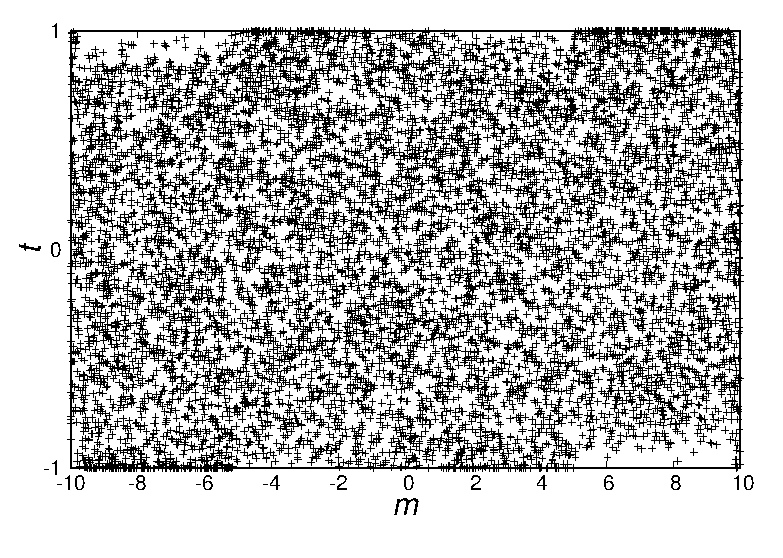
\includegraphics[keepaspectratio,scale=0.33]{minimum_t.eps}
      \end{minipage} \\
      \begin{minipage}{0.50\hsize}
        \centering
        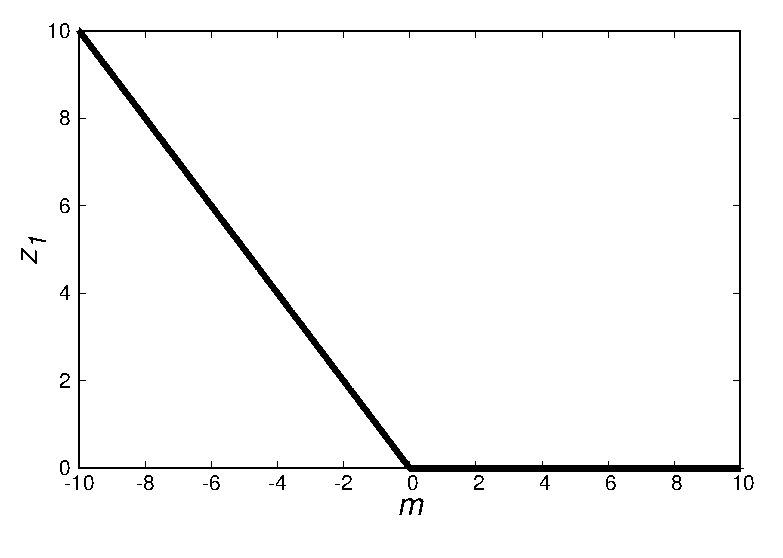
\includegraphics[keepaspectratio,scale=0.33]{minimum_z1.eps}
      \end{minipage}
      \begin{minipage}{0.50\hsize}
        \centering
        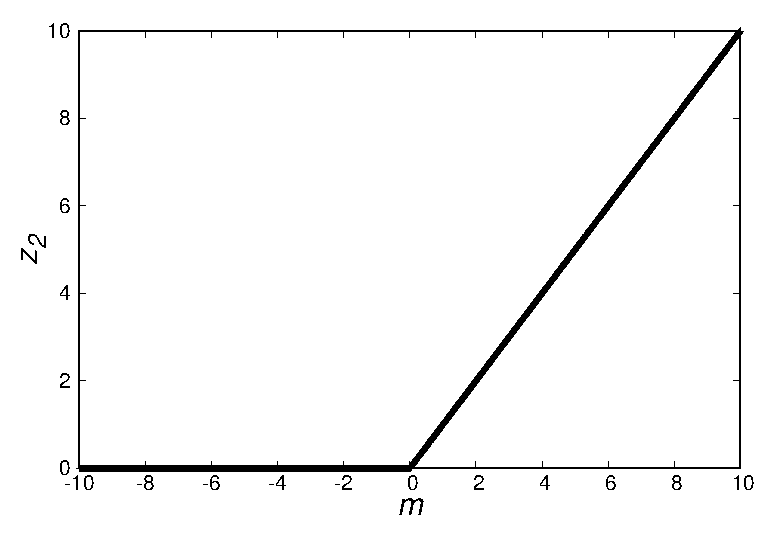
\includegraphics[keepaspectratio,scale=0.33]{minimum_z2.eps}
      \end{minipage}
    \end{tabular}
    \caption{The figures for upper left, upper right, lower left and lower right show the results when $\widetilde{F}(m), t, z_{1}, z_{2}$ are optimized for each $m$ respectively.}
    \label{fig:minimum1}
  \end{center}
\end{figure}

From this result, we can confirm that l1-norm can be obtained by optimizing (\ref{after_wolf}). Also, if we look at each variable $t, z_{1}$ and $z_{2}$ at optimization, we can see the following: It may be possible to reduce one variable by reviewing the (\ref{after_wolf}) because $t$ is not converged alothough $z_{1}$ and $z_{2}$ converge to a specific value.

\section{Reduced QUBO formulation} %定式化の見直し
\subsection{Reduction of the variable in the Legendre transformation}
We can think of the following from the results of the numerical experiments in the previous section: The variable $t$ seems to be taking a random value rather than settling to the optimal value, so we will consider whether we can eliminate $t$ by reviewing the formulation. 
The cost function can be transformed as follows using equality constraint.
\begin{alignat}{2}
  F'(m)&=\min_{t,z_{1},z_{2}}{\{mt+z_{1}(t+1)-z_{2}(t-1)} \nonumber \\
  &\quad+M(-m-z_{1}+z_{2})^{2}\} \nonumber \\
  &=\min_{t,z_{1},z_{2}}{\{mt+z_{1}(t+1)-(m+z_{1})(t-1)} \nonumber \\
  &\quad+M(-m-z_{1}+z_{2})^{2}\} \nonumber \\
  &=\min_{z_{1},z_{2}}{\{z_{1}+(m+z_{1})+M(-m-z_{1}+z_{2})^{2}\}} \nonumber \\
  &=\min_{z_{1},z_{2}}{\{z_{1}+z_{2}+M(-m-z_{1}+z_{2})^{2}\}} \label{review_formulation}
\end{alignat}
This conversion from (\ref{after_wolf}) to (\ref{review_formulation}) is possible because the penalty term, $M(-m-z_{1}+z_{2})^{2}$, forces the equality constraint to be satisfied.

\subsection{Numerical validation} %定式化したものを利用して実験を行う
The result of experimenting the optimization problem under the same experimental conditions as Section\ref{Native_derivation} with (\ref{review_formulation}) as the objective function is as shown in Fig.\ref{fig:minimum2}.

\begin{figure}[htbp]
  \begin{center}
    \begin{tabular}{c}
      \begin{minipage}{0.50\hsize}
        \centering
        \includegraphics[keepaspectratio,scale=0.33]{minimum_cost_non_t.eps}
      \end{minipage} \\
      \begin{minipage}{0.50\hsize}
        \centering
        \includegraphics[keepaspectratio,scale=0.33]{minimum_z1_non_t.eps}
      \end{minipage}
      \begin{minipage}{0.50\hsize}
        \centering
        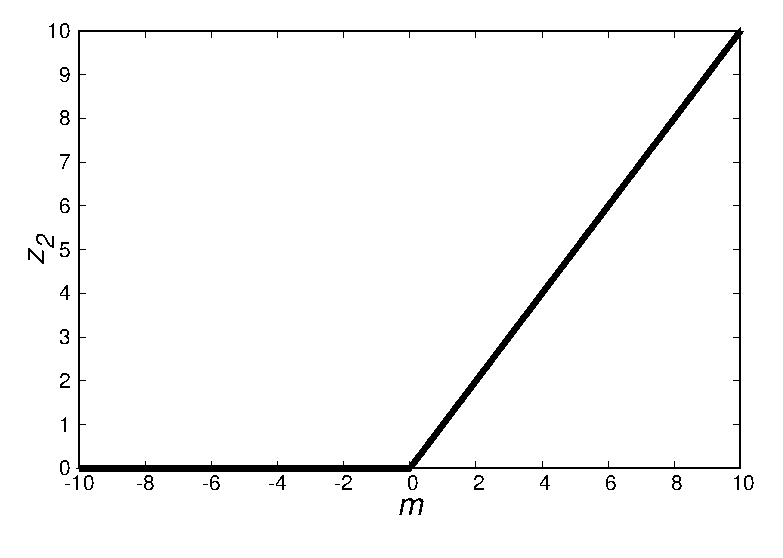
\includegraphics[keepaspectratio,scale=0.33]{minimum_z2_non_t.eps}
      \end{minipage}
    \end{tabular}
    \caption{The figures for upper, lower left and lower right show the results when $\widetilde{F}(m), z_{1}, z_{2}$ are optimized for each $m$ respectively.}
    \label{fig:minimum2}
  \end{center}
\end{figure}
From this result, the outline of $\widetilde{F}(m), z_{1}$ and $z_{2}$ when optimizing (\ref{after_wolf}) did not change from Fig.\ref{fig:minimum2}, so we seem that removing the variable $t$ does not affect the result.


\section{conclsion}
%本稿では, l1-normのQUBO形式での定式化を提案し, 数値実験を通じて変数の削減を行なった. しかし, この変数の削減方法は定式化を見ただけでも予測可能である. また, イジング型マシンでスパース推定をするためにコスト関数にl1-normを追加すると, 各推定値に対してそれぞれ二つの変数を追加する必要があり, 依然として変数の数が多い. はじめに説明したように変数を減らすことはハードウェアへの実装を考える上では重要であり, この定式化にはまだ問題が残っている. この問題の解決法として, 今回の実験では先行研究で用いられた導出法を用いることで導出を行なったが, それとは異なる導出法を用いることで追加で必要になる変数の数を減らすことが可能になるかもしれない. 
In this paper, we propose the formulation of $\ell_{1}$-norm in the QUBO formulation and resuce the variables through numerical experiments. However, the reduction method of this variable can be predicted just by looking at the formulation. When $\ell_{1}$-norm is added to the cost function in order to make sparse estimation with Ising machine, it is necessary to add two variables for each estimated value, and the number of variables is still large. It is important to consider the implementation on hardware, and the problem still remains in this formulaiton. As a solution of this problem, in this experiment, the derivation was performed using the method used in the previous research, but it may be possible to reduce the number of additional variables required by using a different derivation method.

\begin{acknowledgment}

%\acknowledgment

%For enveironments for acknowledgment(s) are available: \verb|acknowledgment|, \verb|acknowledgments|, \verb|acknowledgment|, and \verb|acknowledgments|.

\end{acknowledgment}

%\appndix
%\section{}
%Use the \verb|\appendix| command if you need an appendix(es). The \verb|\section| command should follow even though there is no title for the appendix (see above in the source of this file).
%For authurs of Invited Review Papers, the \verb|profile| command si prepared for the author(s)' profile. A simple example is shown below.

%\begin{verbatim}
%\profile{Taro Butsuri}{was born in Tokyo, Japan in 1965. ...}
%\end{verbatim}

\begin{thebibliography}{1}
\bibitem{d-wave01}
  M. W. Johnson, M. H. S. Amin, S. Gildert, T. Lanting, F. Hamze, N. Dickson, R. Harris, A. J. Berkley, J. Johansson, P. Bunyk, E. M. Chapple, C. Enderud, J. P. Hilton, K. Karimi, E. Ladizinsky, N. Ladizinsky, T. Oh, I. Perminov, C. Rich, M. C. Thom, E. Tolkacheva, C. J. S. Truncik, S. Uchaikin, J. Wang, B. Wilson and G. Rose, Nature. {\bf 473}, 194 (2011).
\bibitem{d-wave02}
  P. I. Bunyk, E. Hoskinson, M. W. Johnson, E. Tolkacheva, F. Altomare, A. J. Berkley, R. Harris, J. P. Hilton, T. Lanting, J. Whittaker, IEEE Trans. Appl. Supercond. {\bf 24}, 1700110 (2014).
\bibitem{DA}
  M. Aramon, G. Rosenberg, E. Valiante, T. Miyazawa, H. Tamura, and H. G. Katzgraber, arXiv:1806.08815.
\bibitem{q-loss}
  V. Denchev, N.Ding, S. V. N Vishwanathan, and H. Neven, in Proceedings of the 29th International Conference on Machine Learning, p.863 (2012).
\bibitem{relu}
  Go Sato, Makiko Konoshima, Takuya Ohwa, Hirotaka Tamura and Jun Ohkubo, arXiv:1911.03829.
\bibitem{wolfe}
  P. Wolfe, Quart. Appl. Math. {\bf 19}, 239 (1961).
\bibitem{lasso}
  Robert Tibshirani, Regression Shrinkage and Selection via the Lasso, J. R. Statist. Soc, B, 58(1):267-288 (1996).
  
\end{thebibliography}

\end{document}

